\chapter{Vorlage}
\section{Text und Formatierung}
Aufzählung
\begin{enumerate}
\item Tausend
\item Tanten
\item Tanzen
\item Tango
\end{enumerate}

Auflistung
\begin{itemize}
\item{Eier und Schmalz}
\item{Zucker und Salz}
\item{Milch und Mehl}
\item{Safran macht den Kuchen gehl}
\end{itemize}

Text in \enquote{Anführungsstrichen} macht man so. Markierter \achtung{Text} z.B. weil noch zu überarbeiten.

\section{Einbindung Bilder}

\begin{figure}[h]
	\centering
	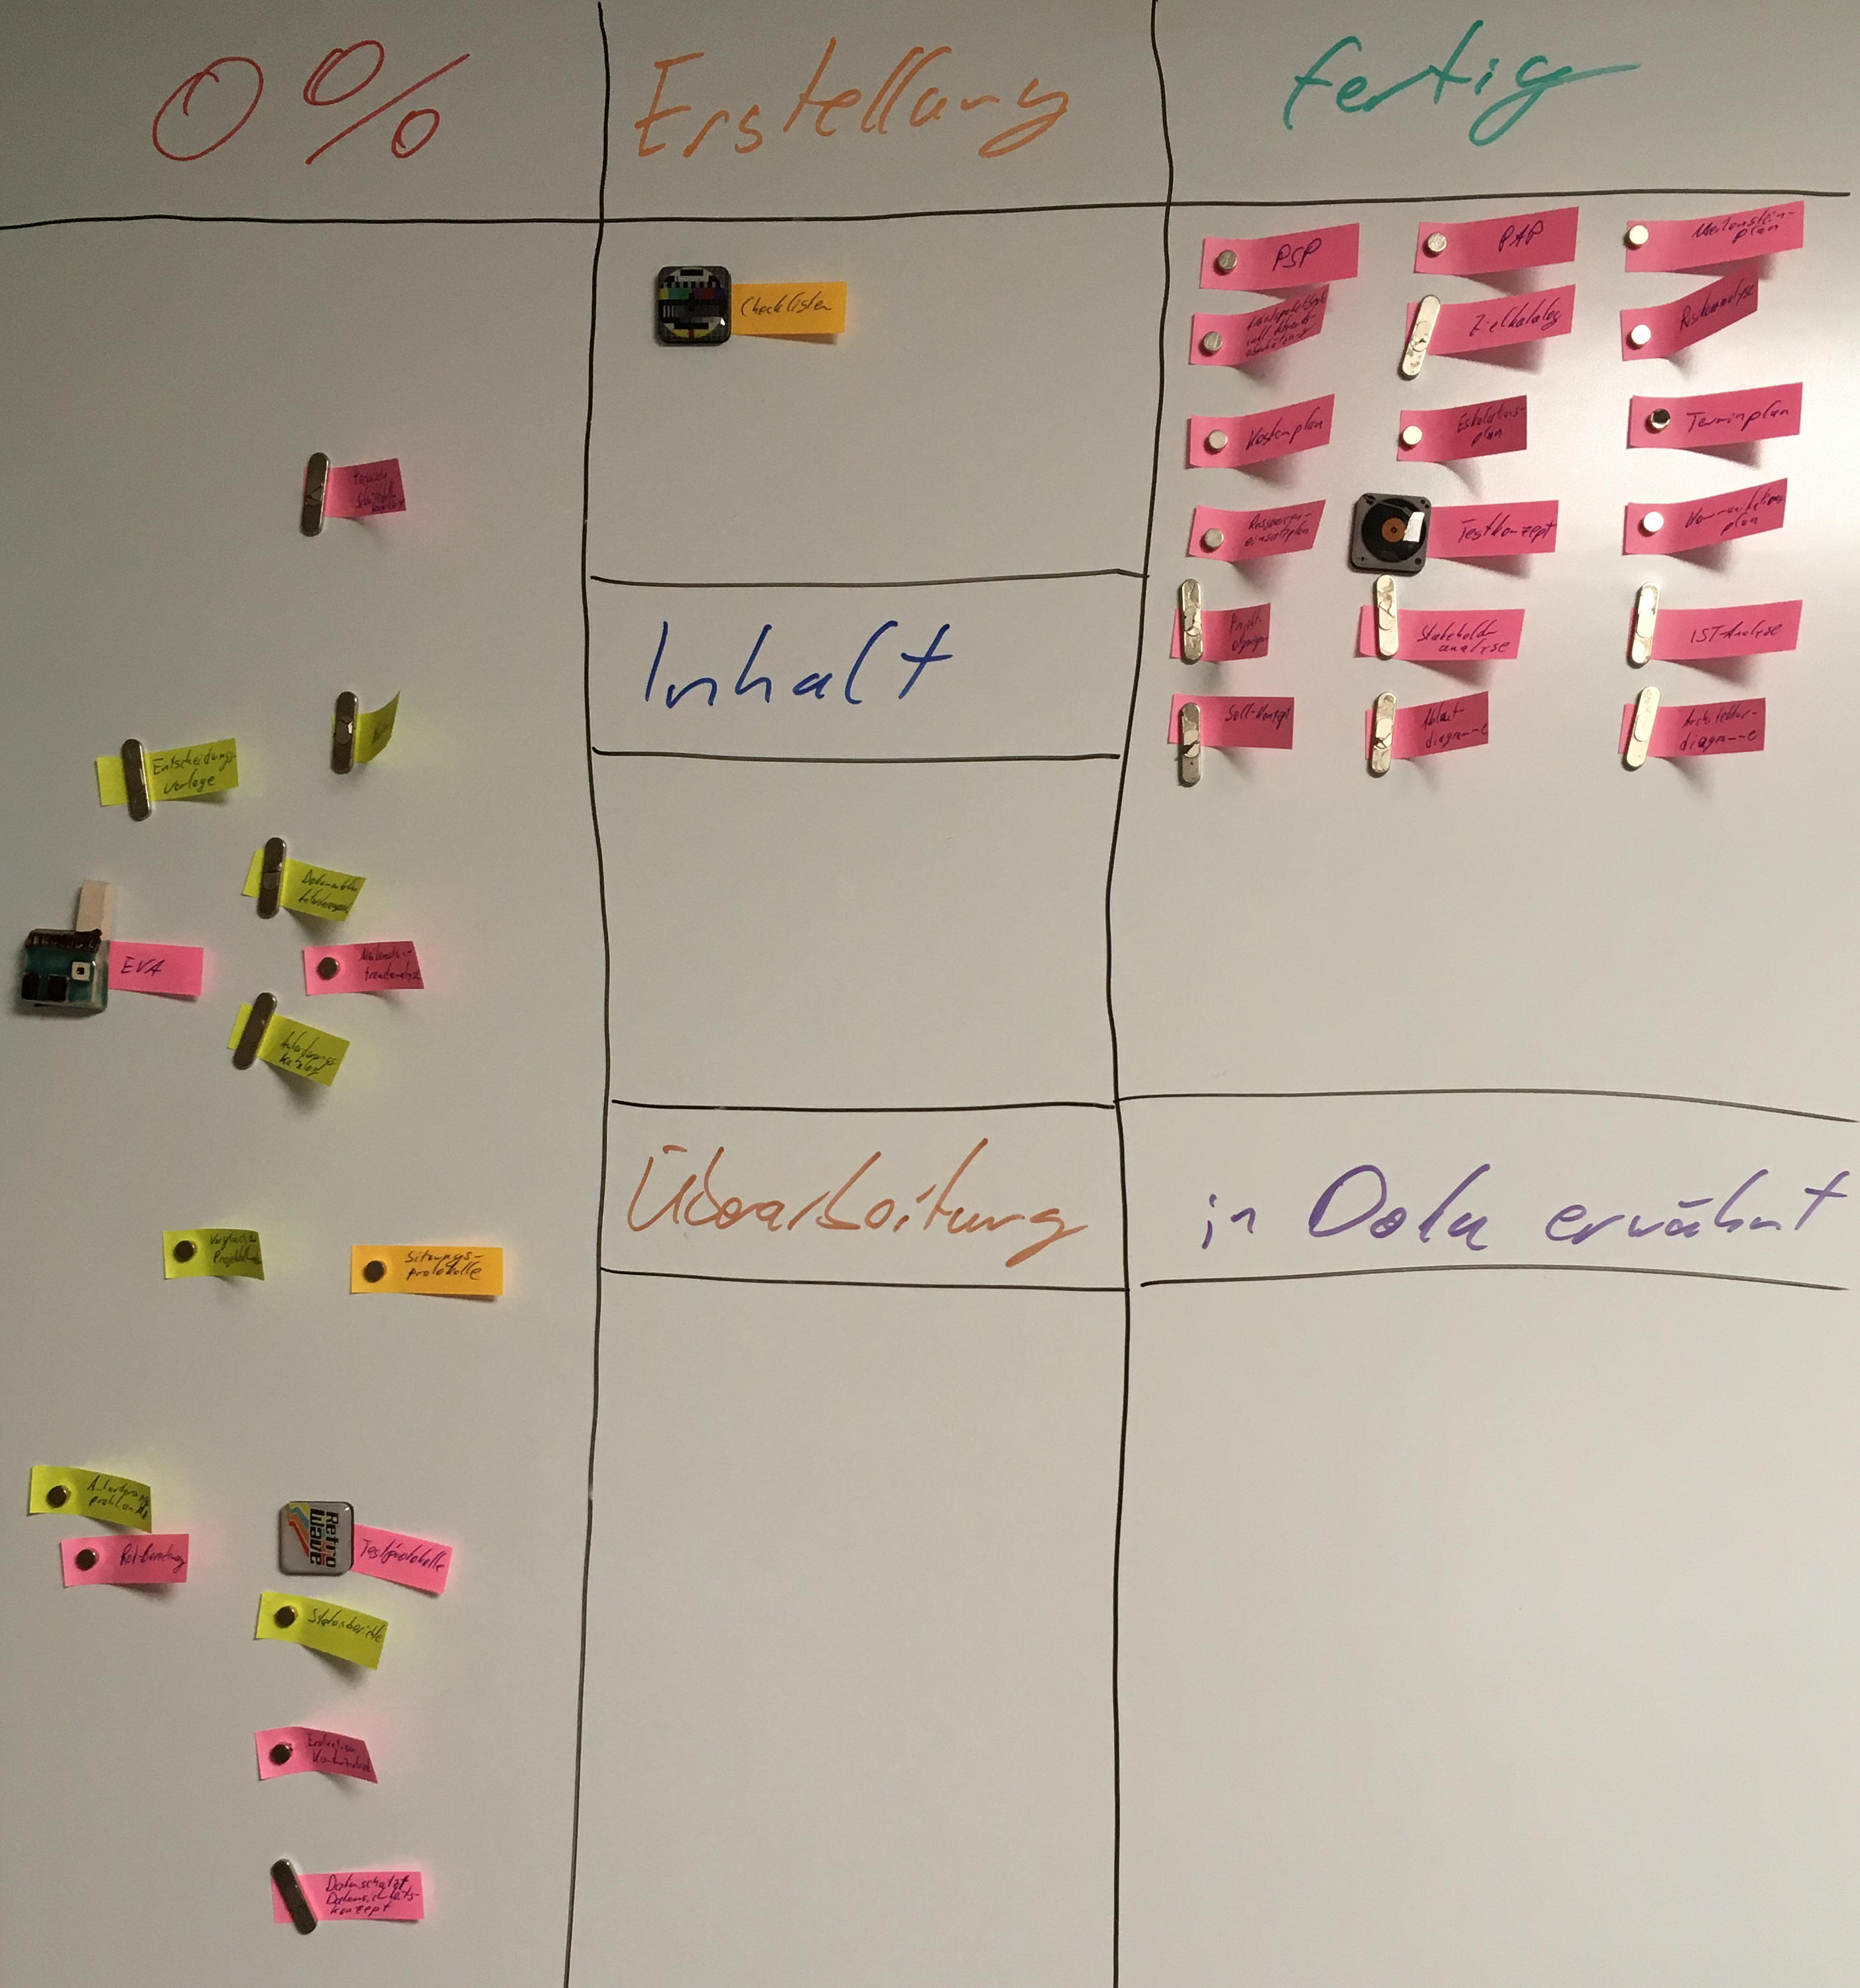
\includegraphics[width=0.85\textwidth]{./pics/kanban.jpg}
	\caption{eingebundenes Bild}
\end{figure}

Das Bild wird automatisch in das entsprechende Verzeichnis aufgenommen.

\section{Hinweis Anhänge}
Bei den Anlagen darauf achten, dass die Seitennummer immer an der richtigen Stelle ist. Also nach dem Ausdruck und der Ringheftung immer unten. Der Titel sollte hingegen immer oberhalb der \enquote{Leserichtung} dargestellt sein. Um zu verhindern, dass sich der Inhalt der Anlagen und die Überschriften der eigentlichen Dokumentation überlagern, kann mit \enquote{offset} und \enquote{scale} gearbeitet werden.